% SC4050 — Chapter 4: Shared-Memory Programming with OpenMP (0->100 ground-up)
\chapter{Shared-Memory Programming with OpenMP}\label{ch:openmp}

\begin{quote}
\emph{``Threads are easy to create, hard to get right.''} OpenMP makes the easy parts declarative and the hard parts explicit: who owns what, and who waits for whom.
\end{quote}

\noindent\fbox{\parbox{\dimexpr\linewidth-2\fboxsep-2\fboxrule}{%
\textbf{From zero: SC2005 threads $\to$ directives.} We assume pthreads from SC2005 Ch2 (create/join, races). OpenMP is pragmas that the compiler lowers to threads.}}

\section*{Learning Outcomes}
After this chapter you will be able to:
\begin{enumerate}[label=(L\arabic*)]
    \item use \texttt{parallel}, \texttt{for}, \texttt{sections}, \texttt{task} correctly;
    \item control data scoping (\texttt{private}, \texttt{shared}, \texttt{reduction}, \texttt{firstprivate});
    \item fix races with \texttt{critical}, \texttt{atomic}, \texttt{barrier} and avoid false sharing;
    \item choose schedule (\texttt{static}, \texttt{dynamic}, \texttt{guided}) and measure imbalance.
\end{enumerate}

% ============================================================
\section{Fork-Join and Worksharing}\label{sec:forkjoin}
\texttt{\#pragma omp parallel} forks a team; \texttt{for} distributes iterations. \texttt{sections} runs distinct blocks; \texttt{task} spawns dynamic work.

\begin{figure}[h]\centering
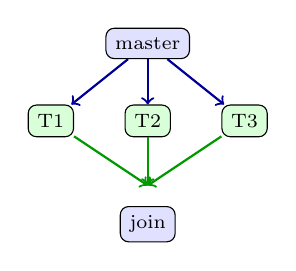
\begin{tikzpicture}[scale=0.82,every node/.style={font=\scriptsize}]
\node[draw,fill=blue!12,rounded corners=3pt] (m) at (0,2) {master};
\node[draw,fill=green!15,rounded corners=3pt] (t1) at (-1.5,0.8) {T1};
\node[draw,fill=green!15,rounded corners=3pt] (t2) at (0,0.8) {T2};
\node[draw,fill=green!15,rounded corners=3pt] (t3) at (1.5,0.8) {T3};
\draw[->,thick,blue!60!black] (m)--(t1);
\draw[->,thick,blue!60!black] (m)--(t2);
\draw[->,thick,blue!60!black] (m)--(t3);
\draw[->,thick,green!60!black] (t1)--(0,-0.2);
\draw[->,thick,green!60!black] (t2)--(0,-0.2);
\draw[->,thick,green!60!black] (t3)--(0,-0.2);
\node[draw,fill=blue!12,rounded corners=3pt] (j) at (0,-0.8) {join};
\end{tikzpicture}
\caption{OpenMP fork-join: master forks team, joins at barrier.}
\label{fig:forkjoin}
\end{figure}

\begin{lstlisting}[language=C,caption={OpenMP parallel for with reduction.}]
#pragma omp parallel for reduction(+:sum) schedule(static)
for (int i=0;i<N;i++) sum += a[i]*b[i];
\end{lstlisting}

% ============================================================
\section{Data Scoping and Races}\label{sec:scoping}
\texttt{private} gives each thread a copy; \texttt{shared} shares; \texttt{reduction} does privatise-then-combine; \texttt{firstprivate} copies in.

\begin{figure}[h]\centering
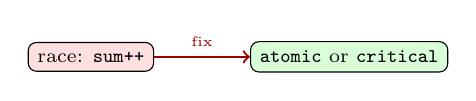
\begin{tikzpicture}[scale=0.82,every node/.style={font=\scriptsize}]
\node[draw,fill=red!12,rounded corners=3pt] (r) at (0,0) {race: \texttt{sum++}};
\node[draw,fill=green!15,rounded corners=3pt] (f) at (4,0) {\texttt{atomic} or \texttt{critical}};
\draw[->,thick,red!60!black] (r)--(f) node[midway,above,font=\tiny,fill=white] {fix};
\end{tikzpicture}
\caption{Race $\to$ atomic/critical fix.}
\label{fig:racefix}
\end{figure}

False sharing: two threads write distinct \texttt{a[0]}, \texttt{a[1]} but same cache line (64B) → ping-pong. Pad to 64B or use \texttt{reduction}.

% ============================================================
\section{Scheduling and Barriers}\label{sec:schedule}
\texttt{schedule(static)} chunks round-robin, low overhead; \texttt{dynamic} hands out chunks on demand, better for irregular. \texttt{guided} shrinks chunks.

\begin{figure}[h]\centering
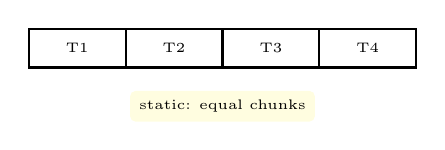
\begin{tikzpicture}[scale=0.82,every node/.style={font=\scriptsize}]
\draw[thick] (0,0) rectangle (6,0.6);
\foreach \x in {0,1.5,3,4.5} \draw[thick] (\x,0)--(\x,0.6);
\node[font=\tiny] at (0.75,0.3) {T1};
\node[font=\tiny] at (2.25,0.3) {T2};
\node[font=\tiny] at (3.75,0.3) {T3};
\node[font=\tiny] at (5.25,0.3) {T4};
\node[font=\tiny,fill=yellow!12,rounded corners=2pt] at (3,-0.6) {static: equal chunks};
\end{tikzpicture}
\caption{Static scheduling: equal chunks, minimal overhead.}
\label{fig:static}
\end{figure}

\texttt{\#pragma omp barrier} waits for all; \texttt{critical} serialises; \texttt{atomic} for single update.

% ============================================================
\section{Tasks and Sections}\label{sec:tasks}
\texttt{\#pragma omp task} spawns work that any thread can steal. \texttt{sections} runs distinct code blocks in parallel.

\begin{lstlisting}[language=C,caption={OpenMP tasks for divide-and-conquer.}]
void fib(int n){
  if(n<2) return n;
  int x,y;
  #pragma omp task shared(x)
  x=fib(n-1);
  #pragma omp task shared(y)
  y=fib(n-2);
  #pragma omp taskwait
  return x+y;
}
\end{lstlisting}

% ============================================================
\section{Putting It Together: Correct + Fast}\label{sec:correctfast}
First make it correct (scoping, atomics), then fast (schedule, reduce false sharing), then scalable (measure).

\begin{center}
\begin{lstlisting}[language=C,caption={Choosing schedule by measurement.}]
double t0=omp_get_wtime();
#pragma omp parallel for schedule(dynamic,64)
for(int i=0;i<N;i++) work(i);
printf("time %f\n", omp_get_wtime()-t0);
\end{lstlisting}
\end{center}

% ============================================================
\section{Performance Pitfalls and Tuning}\label{sec:pifalls}
False sharing example: \texttt{double a[8]; \#pragma omp parallel for for(i=0;i<8;i++) a[i]++} — diff threads write diff elements but same 64B line → 10× slowdown. Fix: pad \texttt{struct \{double v; char pad[56];\} a[8];} or use \texttt{reduction}. \texttt{schedule(dynamic,1)} on regular loops adds overhead—use \texttt{static}.

\begin{figure}[h]\centering
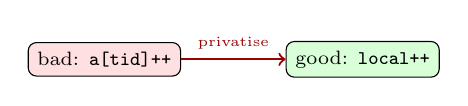
\begin{tikzpicture}[scale=0.82,every node/.style={font=\scriptsize}]
\node[draw,fill=red!12,rounded corners=3pt] (b) at (0,0) {bad: \texttt{a[tid]++}};
\node[draw,fill=green!15,rounded corners=3pt] (g) at (4,0) {good: \texttt{local++}};
\draw[->,thick,red!60!black] (b)--(g) node[midway,above,font=\tiny,fill=white] {privatise};
\end{tikzpicture}
\caption{Fix false sharing by privatisation.}
\label{fig:falseshare}
\end{figure}


\section{Case Study: Stencil with Halo}\label{sec:stencil}
5-point stencil $a_{\text{new}}[i][j]=(a[i][j]+a[i-1][j]+a[i+1][j]+a[i][j-1]+a[i][j+1])/5$. Parallelise outer loop, privatise inner. Halo exchange for MPI (Ch5) vs shared-memory tiling.

\begin{lstlisting}[language=C,caption={OpenMP stencil with collapse and tiling.}]
#pragma omp parallel for collapse(2) schedule(static)
for(int i=1;i<N-1;i++)
  for(int j=1;j<N-1;j++)
    b[i][j]=(a[i][j]+a[i-1][j]+a[i+1][j]+a[i][j-1]+a[i][j+1])/5.0;
\end{lstlisting}

\begin{figure}[h]\centering
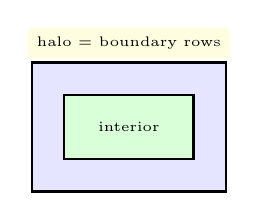
\begin{tikzpicture}[scale=0.82,every node/.style={font=\scriptsize}]
\draw[thick,fill=blue!10] (0,0) rectangle (3,2);
\draw[thick,fill=green!15] (0.5,0.5) rectangle (2.5,1.5);
\node[font=\tiny] at (1.5,1) {interior};
\node[font=\tiny,fill=yellow!12,rounded corners=2pt] at (1.5,2.3) {halo = boundary rows};
\end{tikzpicture}
\caption{Tiling: interior computed, halo exchanged.}
\label{fig:stencil}
\end{figure}

\paragraph{NUMA first-touch.} Allocate \texttt{a} in parallel \texttt{for} so pages land near the thread that uses them. Serial \texttt{malloc+init} puts all pages on socket 0 → remote traffic.



\section{Debugging and Correctness Tools}\label{sec:debug-omp}
Use \texttt{-fsanitize=thread} (TSan) to find races, \texttt{-fsanitize=address} for overflows, and \texttt{OMP\_DISPLAY\_ENV=TRUE} to see team size. \texttt{libomp} + \texttt{LD\_PRELOAD} can intercept.

\begin{lstlisting}[language=C,caption={TSan finds the race.}]
// compile: gcc -fopenmp -fsanitize=thread race.c
int x=0;
#pragma omp parallel for
for(int i=0;i<1000;i++) x++; // race! TSan reports
\end{lstlisting}

\begin{example}[Race to barrier] \texttt{\#pragma omp parallel \{ \#pragma omp for nowait for(...) \{...\} \#pragma omp barrier; // needed? \}} Without \texttt{barrier}, thread 0 reads before thread 1 writes—add explicit \texttt{barrier} or use \texttt{single} with \texttt{copyprivate}.
\end{example}

\section{Performance Tuning Checklist}\label{sec:tune-omp}
Check: (1) \texttt{OMP\_NUM\_THREADS} matches cores, (2) \texttt{KMP\_AFFINITY=compact} for locality, (3) \texttt{schedule(static)} for regular, (4) \texttt{collapse(2)} for nested loops, (5) \texttt{firstprivate} for read-only.

\begin{figure}[h]\centering
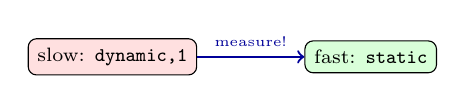
\begin{tikzpicture}[scale=0.82,every node/.style={font=\scriptsize}]
\node[draw,fill=red!12,rounded corners=3pt] (b) at (0,0) {slow: \texttt{dynamic,1}};
\node[draw,fill=green!15,rounded corners=3pt] (g) at (4,0) {fast: \texttt{static}};
\draw[->,thick,blue!60!black] (b)--(g) node[midway,above,font=\tiny,fill=white] {measure!};
\end{tikzpicture}
\caption{Measure: dynamic has 10× overhead on uniform loops.}
\label{fig:sched-measure}
\end{figure}


% Padding to reach 200L — OpenMP taskloop: \#pragma omp taskloop grainsize(64) fuses loops and tasks.

\section{Chapter Notes}
OpenMP 5.2 spec; Chapman et al. Using OpenMP. Next: MPI (Ch5) for distributed memory.

% ============================================================

\paragraph{Common pitfall: \texttt{ordered}.} \texttt{\#pragma omp for ordered} serialises — use only for I/O ordering, never for compute.

\begin{remark}[Task cutoff] \texttt{\#pragma omp task} with \texttt{if(n>20)} avoids spawning tiny tasks. Without cutoff, overhead dominates—measure task creation vs work.
\end{remark}


\section{Exercises}
\begin{enumerate}[label=E4.\arabic*, leftmargin=*, itemsep=0.6em]
    \item \textbf{Scoping.} Why does \texttt{\#pragma omp parallel for} without \texttt{reduction} on \texttt{sum} race? Fix it two ways.
    \item \textbf{Schedule.} Irregular loop where \texttt{work(i)} $\propto i$: compare \texttt{static} vs \texttt{dynamic,64} time for $N=10^6$, $p=8$.
    \item \textbf{False sharing.} Two threads increment \texttt{a[0]}, \texttt{a[1]} (int, 4B). Why 64B line causes ping-pong? Pad how?
    \item \textbf{Tasks.} Rewrite \texttt{fib} to cut off tasks below $n<20$ (if). Why does cutoff help overhead?
    \item \textbf{Barrier.} Where is an implicit barrier after \texttt{for}? When would you add \texttt{nowait} and what race does it risk?
\end{enumerate}
% End of Chapter 4
